%! Author = adrienkoumgangtegantchouang
%! Date = 07/06/25


% Preamble
\documentclass[a4paper, 12pt]{report}
\usepackage[osf]{libertinus}
\pagestyle{plain}
\usepackage[top=2.5cm,bottom=2.5cm,left=4cm,right=2.5cm, centering]{geometry}
\linespread{1.5}
\usepackage[utf8]{inputenc} % codifica UTF-8
\usepackage{scrlayer-scrpage} % stili pagina per il frontespizio
\pagestyle{scrplain}
\usepackage{mathptmx} % font Times New Roman (simile)
\usepackage{graphicx, wrapfig}
\usepackage{lipsum}

\usepackage{url}
\usepackage{changepage}
\usepackage{multicol}
\usepackage{caption}
\usepackage{subcaption} % For the images' captions
\usepackage[linesnumbered,ruled,vlined]{algorithm2e}
\usepackage{amsmath} % For math symbols
\usepackage{amsthm} % Theorem styles
\usepackage{amssymb} % For special symbols % \mathbb and others
\usepackage{mathrsfs} % An alternative font for categories and sheaves.
\usepackage{cite} % For multiple citations
% \usepackage{caption}
% \usepackage{subcaption} % For the images' captions
\usepackage[section]{placeins} % To not break (sub)-images in two
\usepackage{booktabs}
\usepackage{float} % Always for images
\usepackage{soul} % For the \ul command, to use lists with less vertical spacing
\usepackage{enumerate} % For (i) list style
\usepackage{glossaries}
% \usepackage{minted}

\usepackage{blindtext}
\usepackage{hyperref}

%\usepackage{biblatex} % Imports biblatex package
%\addbibresource{mybibliography.bib} % Import the bibliography file

\usepackage{listings}
% \usepackage{listings-rust}
% \usepackage{rustlistings}
\usepackage{xcolor} % Optional: for colored code
\renewcommand{\lstlistingname}{Code}% Listing -> Codice\renewcommand{\lstlistingname}{Code}% Listing -> Codice

\usepackage[noend]{algpseudocode}
\algnewcommand\algorithmicforeach{\textbf{for each}}
\algdef{S}[FOR]{ForEach}[1]{\algorithmicforeach\ \#1 \algorithmicdo}

% \usepackage{color}
\usepackage{ragged2e}
\usepackage{algorithmicx}
% \usepackage{algorithm}
% \usepackage{algorithm2e}
\usepackage{program}
% \usepackage{listings-rust}
\usepackage{mathtools}



% \usepackage{xcolor}
\definecolor{codegreen}{rgb}{0,0.6,0}
\definecolor{codegray}{rgb}{0.5,0.5,0.5}
\definecolor{codemauve}{rgb}{0.4,0.,0.4}
% \definecolor{codepurple}{rgb}{0.5,0.5,0.5}
% \definecolor{backcolour}{rgb}{0.95,0.95,0.92}

% Define a custom color
\definecolor{backcolour}{rgb}{0.95,0.95,0.92}
\definecolor{codegreen}{rgb}{0,0.6,0}
\definecolor{codekeywork3}{rgb}{0.82,0.56,0.43}
% Define a custom style


\lstdefinestyle{python}{
    language=Python,                    % Set language to Python
    basicstyle=\ttfamily\footnotesize,   % Basic font style for the code
    keywordstyle=\color{blue}\bfseries,  % Style for keywords
    stringstyle=\color{red},             % Style for strings
    commentstyle=\color{gray}\itshape,   % Style for comments
    numberstyle=\tiny\color{gray},       % Style for line numbers
    backgroundcolor=\color{backcolour},   % choose the background color
    numbers=left,                        % Show line numbers on the left
    stepnumber=1,                        % Line numbers every 1 line
    numbersep=8pt,                       % Space between line numbers and code
    tabsize=4,                           % Width of a tab
    showspaces=false,                    % Don't show spaces
    showstringspaces=false,              % Don't show spaces in strings
    showtabs=false,                      % Don't show tab characters
    frame=single,                        % Add a frame around the code
    rulecolor=\color{black},             % Frame color
    captionpos=b,                        % Position of caption (bottom)
    breaklines=true,                     % Automatically break long lines
    breakatwhitespace=true,              % Allow breaking at whitespace
    backgroundcolor=\color{white},       % Set background color
    morekeywords={self, None, True, False}, % Additional Python-specific keywords
    % escapeinside={(*@}{@*)},             % Escape inside code
    alsoother={\<},
    alsoother={\>},
    literate={\<}{{\textless}}1 {\>}{{\textgreater}}1, % Handle < and > symbols
}

\definecolor{jsonbackground}{RGB}{245,245,244}
\definecolor{jsonstring}{RGB}{173,0,0}
\definecolor{jsonkey}{RGB}{0,0,180}
\definecolor{jsoncomment}{RGB}{85,85,85}
\definecolor{jsonnumber}{RGB}{128,64,0}

\lstdefinelanguage{json}{
    basicstyle=\ttfamily\footnotesize,
    numbers=left,
    numberstyle=\tiny\color{gray},
    stepnumber=1,
    numbersep=8pt,
    showstringspaces=false,
    breaklines=true,
    frame=single,
    backgroundcolor=\color{jsonbackground},
    string=[s]{"}{"},
    comment=[l]{//},
    morecomment=[s]{/*}{*/},
    literate=
        *{:}{{{\color{black}:}}}{1}
        {,}{{{\color{black},}}}{1}
        {\{}{{{\color{black}{\{}}}}{1}
        {\}}{{{\color{black}{\}}}}}{1}
        {[}{{{\color{black}[}}}{1}
        {]}{{{\color{black}]}}}{1}
    keywordstyle=\color{jsonkey}\bfseries,
    stringstyle=\color{jsonstring},
    commentstyle=\color{jsoncomment}\itshape
}


\newtheorem{mydef}{Definition}
\newtheorem{mytheo}{Theorem}
\newtheorem{mylem}{Lemma}
\newtheorem{mypro}{Property}
\newtheorem{myex}{Example}
\newtheorem{mycor}{Corollary}
\newtheorem{myproof}{Proof idea}
\newtheorem{mypc}{Pseudocode}



\begin{document}
    %! Author = adrienkoumgangtegantchouang
%! Date = 07/06/25

\begin{titlepage} %crea l'enviroment
\begin{figure}[t] %inserisce le figure
    \centering
\includegraphics[width=0.70\textwidth]{marchio_unipi_pant541}\label{fig:figure-first-page}
\end{figure}

\begin{figure}[t] %inserisce le figure
    \centering
\includegraphics[width=0.60\textwidth]{DII Logo}\label{fig:figure-first-page-2}
\end{figure}

\vspace{5mm}

\begin{Large}
 \begin{center}
	\textbf{Master's Degree in Artificial Intelligence and Data Engineering\\}
	\vspace{7mm}
    {\Large{Design and develop of an Application interacting with NoSQL Databases:}}\\
	\vspace{2mm}
	{\LARGE{\textbf{Smart News Aggregator}}}
\end{center}
\end{Large}

\vspace{10mm}

%minipage divide la pagina in due sezioni settabili
\begin{minipage}[t]{0.47\textwidth}
	{\large{\textbf{Instructors:\\ Prof. Pietro Ducange \\ Prof. Alessio Schiavo}}}
\end{minipage}
\hfill
\begin{minipage}[t]{0.47\textwidth}\raggedleft
	{\large{\textbf{Student: \\ Adrien Koumgang Tegantchouang}}}
\end{minipage}

\vspace{20mm}

\centering{\large{\textbf Academic Year 2024/2025}}

\end{titlepage}


    \tableofcontents


    \thispagestyle{empty}

    \clearpage
    \setcounter{page}{1}


% Introduction
    %! Author = adrienkoumgangtegantchouang
%! Date = 08/06/25


\chapter{Introduction}\label{ch:introduction}


\section{Overview}\label{sec:overview}

In the digital age, the volume of news articles produced every day is staggering.
Readers are increasingly overwhelmed by the amount of available content and often struggle to find reliable and relevant information that matches their personal interests.
To address this challenge, we propose the development of a \textbf{Smart News Aggregator & Reader Personalization Platform}.

This platform collects news articles from multiple external APIs, stores and processes them using NoSQL databases (MongoDB and Redis), and delivers a personalized reading experience to users.
It incorporates intelligent recommendation features, secure user authentication via JWT tokens, and real-time analytics to improve user engagement.


\section{Objectives}\label{sec:objectives}

The primary objective of this project is to \textbf{design and implement a distributed news aggregation application} of intelligently retrieving,
storing, analyzing, and serving large-scale multi-structured data using multiple NoSQL database technologies.

In line with the course requirements for \textbf{Large Scale and Multi-Structured Databases}, the specific goals of this project include:

\begin{itemize}
    \item \textbf{Data Acquisition \& Preprocessing}: Retrieve a real-world, high-volume dataset ($\leg$ 50MB) from multiple external news APIs (e.g., MediaStack, newsData, The Guardian, NYTimes), ensuring \textbf{variety} and \textbf{velocity}.
    \item \textbf{Distributed NoSQL Architecture}: Use \textbf{MongoDB} as the primary \textbf{Document Database}, with carefully designed collections, indexes, and aggregation pipelines.
    Integrate a \textbf{Key-Value store} (\textbf{Redis}) to optimize caching and access to hot data.
    \item \textbf{System Design and Modeling}: Define functional and non-functional requirements.
    Design UML class diagrams and user interface mockups.
    Model the data schema for each NoSQL DB in use.
    \item \textbf{RESTful API Backend}: Build a scalable backend using Flask and Flask-RESTX.
    Expose secure endpoints with JWT-based authentication.
    Provide API documentation via Swagger and test interfaces.
    \item \textbf{Advanced Analytics}: Implement at least three real aggregation pipelines in MongoDB for summarizing and analyzing article content and user activity.
    Provide user-personalized views and filtering using advanced queries.
    \item \textbf{Monitoring, Testing, and Depployment}: Deploy on both and UNIPI virtual clusters.
    Include performance tests, system logging, and analysis of read/write throughput under different consistency models.
    Offer a complete presentation and demonstration, including API functionality and analytics insights.
\end{itemize}

By achieving these goals, the project demonstrates my ability to handle real-world large-scale data applications,
integrating theoretical design with practical deployment, and ensuring cross-database consistency and performance.


\section{Structure of the presentation}\label{sec:structure-of-the-presentation}

The documentation is structured as follows:

\begin{itemize}
    \item \textbf{Chapter 1 - Introduction}: Presents the context, objectives, and structure of the project, outlining the motivations and academic scope.
    \item \textbf{Chapter 2 - Requirements Analysis}: Identifies the functional and non-functional requirements of the application, defines the system actors, and outlines key use cases.
    \item \textbf{Chapter 3 - System Design}: Includes the architectural overview, UML class diagrams, and mockup wireframes of the application’s user interface.
    \item \textbf{Chapter 4 - NoSQL Database Modeling}: Describes the design choices for MongoDB (Document DB) and Redis (Key-Value DB), along with schema definitions, key structures, and CAP theorem considerations.
    \item \textbf{Chapter 5 - Data Ingestion and Integration}: Explains how external APIs are connected, data is fetched and transformed, and stored into the databases.
    Also includes logging and handling of errors and API rate limits.
    \item \textbf{Chapter 6 - Backend Implementation}: Details the development of RESTful API endpoints using Flask and Flask-RESTX, JWT authentication, Swagger documentation, and the modular blueprint structure.
    \item \textbf{Chapter 7 - Advanced Aggregations and Analytics}: Presents non-trivial aggregation pipelines in MongoDB, user-specific personalization features, and analytics insights extracted from the dataset.
    \item \textbf{Chapter 8 - Deployment and Testing}: Discusses deployment on local and virtualized environments, performance testing scenarios, and consistency benchmarking across NoSQL systems.
    \item \textbf{Chapter 9 - Conclusion}: Summarizes achievements, reflects on encountered challenges, and suggests possible extensions to improve scalability, interactivity, and intelligence.
\end{itemize}



% Requirements Analysis
    %! Author = adrienkoumgangtegantchouang
%! Date = 08/06/25


\chapter{Requirements Analysis}\label{ch:requiremnts-analysis}


\section{Problem Statement}\label{sec:problem-statement}

With the exponential growth of online content, users are overwhelmed by the volume of news available across platforms.
This leads to difficulty in identifying relevant and trustworthy information.
The proposed system aims to aggregate articles from various news APIs and personalize the reading experience based on user behavior and preferences, while maintaining scalability and high performance.


\section{Stackeholders and Actors}\label{sec:stackeholders-actors}

The successful deployment and functioning of the Smart News Aggregator \& Reader Personalization Platform depends on multiple stakeholders and actors who interact directly or indirectly with the system.
This section outlines their roles and responsibilities.

\subsection{Stackeholders}\label{subsec:stackeholders}

\begin{itemize}
    \item \textbf{End Users}: Consume and interact with news content; expect personalized and relevant information.
    \item \textbf{Platform Administrator}: Oversees user activity, ensures data integrity, and manages access or moderation tasks.
    \item \textbf{Project Developers}: Build and maintain the system backend, frontend, and data processing pipelines.
    \item \textbf{External API Providers}: Supply news content (e.g., NYTimes, Guardian, NewsData, CurrentsAPI, MediaStack).
    \item \textbf{Academic Supervisors}: Oversee the project's architecture, correctness, and evaluate its educational objectives.
\end{itemize}

\subsection{Actors}\label{subsec:actors}

\begin{itemize}
    \item \textbf{Visitor (Anonymous user)}: Accesses the welcome page and Can register to become a user.
    \item \textbf{Registered User}: Logs into the platform, Personalizes preferences, Views news feed and Interacts with articles (like/comment).
    \item \textbf{Administrator}: Manages users and platform configurations and Monitors logs and analytics.
    \item \textbf{News Aggregator Service}: Fetches articles from external APIs and Normalizes and stores them into MongoDB.
    \item \textbf{External News APIs}: Provide raw article data in JSON format for ingestion by the system.
\end{itemize}

Each actor has specific actions and permissions that are further detailed in the Use Case and UML Diagrams.


\section{Functional Requirements}\label{sec:functional-requirments}

The Smart News Aggregator \& Reader Personalization Platform offers a suite of functionalities that serve both user-facing and administrative purposes.
The following functional requirements have been identified:

\subsection{User Account Management}\label{subsec:user-account-management}

\begin{itemize}
    \item \textbf{Registration}: Users must be able to register with valid email and password.
    \item \textbf{Login/Logout}: Authenticated access via JWT-based login; logout clears session on frontend.
    \item \textbf{Profile Management}: Users can update personal data (e.g., name, preferences).
    \item \textbf{Password Handling}: Secure password storage and update with history tracking.
\end{itemize}

\subsection{News Aggregation \& Display}\label{subsec:news-aggregation-diplay}

\begin{itemize}
    \item \textbf{Fetch Articles from External APIs}: The system retrieves and normalizes article data from third-party providers such as NYTimes, NewsData, CurrentsAPI, etc.
    \item \textbf{Categorized News Display}: Articles are displayed by category (e.g., politics, tech, sports).
    \item \textbf{Search \& Filter}: Users can search articles using keywords and filter by category, source, or date.
    \item \textbf{Pagination}: Article lists are paginated to handle large datasets.
\end{itemize}

\subsection{Personalization \& Recommendation}\label{subsec:personalization-recommendation}

\begin{itemize}
    \item \textbf{Save Preferences}: Users can set preferred categories, sources, or languages.
    \item \textbf{Personalized Feed}: Articles are filtered and ranked based on user preferences.
    \item \textbf{Like \& Save Articles}: Users can like or save articles for future reading.
    \item \textbf{Commenting System}: Users can add comments and replies to articles.
\end{itemize}

\subsection{Admin \& Analytics}\label{subsec:admin-analytics}

\begin{itemize}
    \item \textbf{Dashboard Access}: Admin can view usage statistics and system logs.
    \item \textbf{User Management}: Admin can deactivate or delete user accounts.
    \item \textbf{API Health Monitoring}: Admin is notified of errors when external APIs fail.
    \item \textbf{Article Quality Control}: Admin can remove duplicated or malformed articles.
\end{itemize}

\subsection{System \& Logging}\label{subsec:system-logging}

\begin{itemize}
    % \item \textbf{API Logging}: All requests to critical endpoints are logged (including metadata like headers and response time).
    \item \textbf{Authentication Event Logs}: Login/Logout attempts are store for audit.
    \item \textbf{Error Tracking}: Failed requests or errors are stored in MongoDB.
\end{itemize}


\section{Non-Functional Requirements}\label{sec:non-functional-requirements}

This section outlines the quality attributes and constraints the Smart News Aggregator \& Reader Personalization Platform must meet to ensure reliability, security, and scalability.

\subsection{Performance}\label{subsec:performance}

The system must handle a high number of concurrent users with minimal latency.
Article feed pages must load within 1 second under normal network conditions.
External API data must be cached using Redis to reduce response time and load.


\subsection{Scalability}\label{subsec:scalability}

The backend architecture must support horizontal scaling to accommodate growing numbers of users and API integrations.
MongoDB and Redis must be configured to handle large-scale document and key-value datasets efficiently.

\subsection{Availability}\label{subsec:availability}

The application must ensure high availability (99.9\%) during user access hours.
In the case of third-party API failure, the system should provide fallback responses or cached data when available.

\subsection{Security}\label{subsec:security}

User authentication must use JWT with asymmetric encryption (RS256).
Passwords must be securely hashed (using bcrypt) and stored with history to prevent reuse.
All endpoints must enforce token validation for sensitive operations.
Cross-Origin Resource Sharing (CORS) must be properly configured to restrict access to allowed domains.

\subsection{Maintainability}\label{subsec:maintainability}

The system must be modular, separating concerns by feature (auth, articles, users).
Logging and exception handling must be centralized to simplify debugging and maintenance.
Code must be written following best practices and TypeScript (frontend) and Python (backend) style guides.

\subsection{Usability}\label{subsec:usability}

The frontend must offer an intuitive user interface with minimal learning curve.
Responsive design must ensure accessibility on desktops, tablets, and mobile devices.

\subsection{Portability}\label{subsec:portability}

The application must run on Unix-based systems and be container-ready (Docker-compatible).
APIs must be documented using Swagger/OpenAPI to allow easy integration by external systems.


\section{Use Case Diagrams}\label{sec:use-case-diagrams}

These diagrams were created using PlantUML\@.

%\begin{figure}[!h]
%    \centering
%    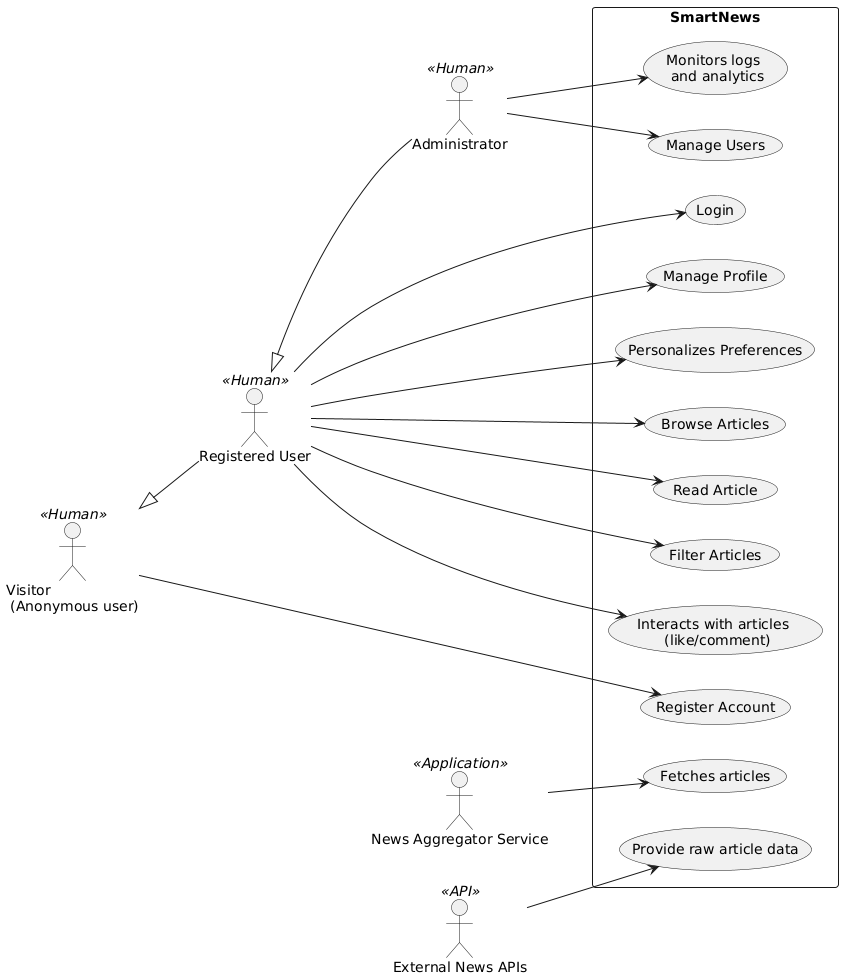
\includegraphics[width=1.1\textwidth]{chapters/chapter_02/diagram-sn-uml-2}
%    \caption{Use Case Diagram}
%    \label{fig:use-case-diagram}
%\end{figure}


\begin{figure}[!h]
    \centering
    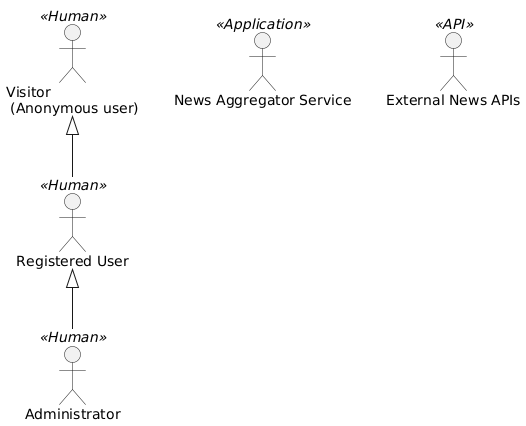
\includegraphics[width=0.5\textwidth]{chapters/chapter_02/use-case-smart-news-actors}
    \caption{Use Case Diagram : Actors}
    \label{fig:use-case-diagram-actors}
\end{figure}


\begin{figure}[!h]
    \centering
    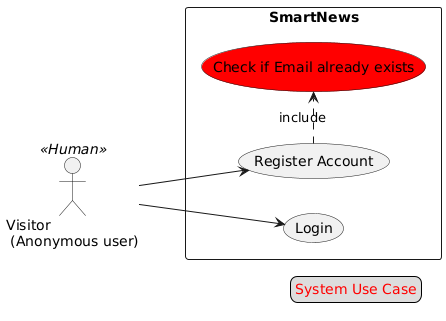
\includegraphics[width=0.5\textwidth]{chapters/chapter_02/use-case-smart-news-anonymous-user}
    \caption{Use Case Diagram: Anonymous User}
    \label{fig:use-case-diagram-anonymous-user}
\end{figure}


\begin{figure}[!h]
    \centering
    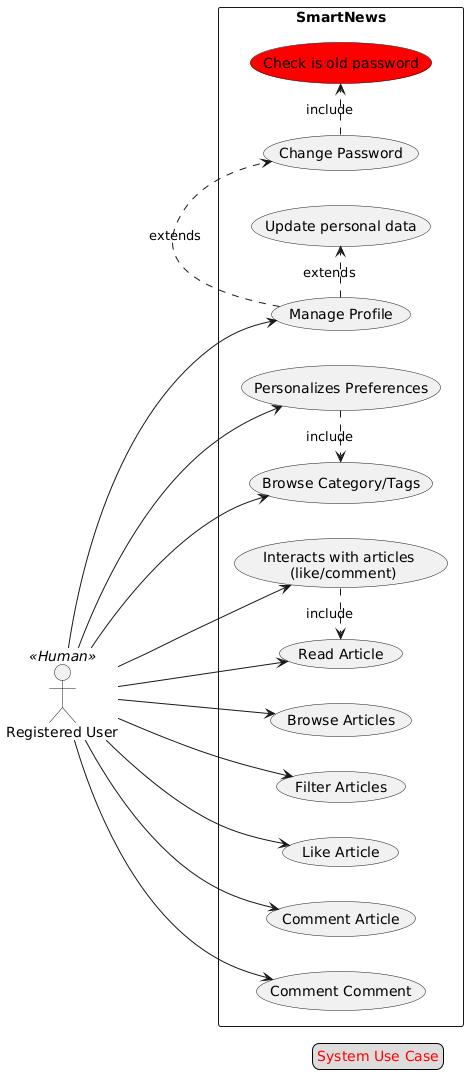
\includegraphics[width=0.5\textwidth]{chapters/chapter_02/use-case-smart-news-registered-user}
    \caption{Use Case Diagram: Registered User}
    \label{fig:use-case-diagram-registered-user}
\end{figure}


\begin{figure}[!h]
    \centering
    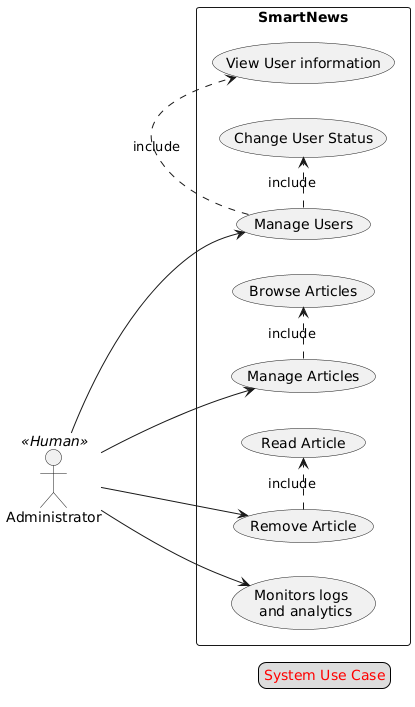
\includegraphics[width=0.5\textwidth]{chapters/chapter_02/use-case-smart-news-administrator}
    \caption{Use Case Diagram: Administrator}
    \label{fig:use-case-diagram-administrator}
\end{figure}


\begin{figure}[!h]
    \centering
    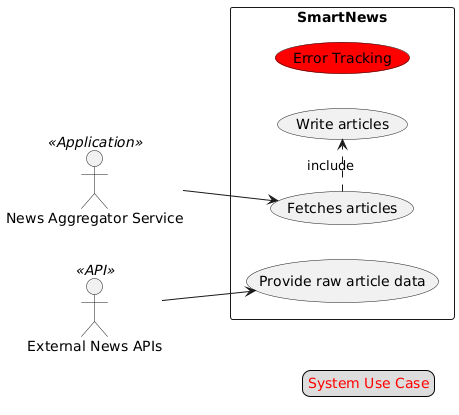
\includegraphics[width=0.5\textwidth]{chapters/chapter_02/use-case-smart-news-system}
    \caption{Use Case Diagram: Systen}
    \label{fig:use-case-diagram-system}
\end{figure}





% System Design
    %! Author = adrienkoumgangtegantchouang
%! Date = 08/06/25


\chapter{System Design}\label{ch:system-design}


This chapter presents the architectural and structural design of the Smart News Aggregator \& Reader Personalization Platform.
It includes a high-level system architecture, database modeling strategy, UML class diagrams, and mockups of key user interfaces.


\section{Architecture Overview}\label{sec:architecture-overview}

The platform is built using a \textbf{modular and layered architecture} to separate concerns and ensure maintainability, performance, and scalability.
It integrates multiple technologies:

\subsection{Key Components}\label{subsec:key-components}

\begin{itemize}
    \item \textbf{Frontend (React\cite{react, vite} + TypeScript)}: Handles UI, user interaction, API communication and Token-based authentication.
    \item \textbf{Backend (Flask + Flask-RESTX)}: RESTful API with Blueprint organization, JWT authentication with RS256 and Logging and error handling.
    \item \textbf{Document Database (MongoDB)}: Stores user profiles, articles, comments, and logs.
    Supports complex queries and aggregation pipelines.
    \item \textbf{Key-Value Store (Redis)}: Caches trending articles and recent queries.
    Session tracking.
    \item \textbf{External APIs}: Article data sources such as CurrentsAPI, NewsData, NYTimes, Guardian.
\end{itemize}


\section{System Architecture Diagram}\label{sec:system-architecture-diagram}

The architecture is divided into four layers:
\begin{itemize}
    \item \textbf{Client Layer}: Browser-based React frontend
    \item \textbf{Application Layer}: Flask server handling HTTP requests, routing, and validation
    \item \textbf{Data Layer}: MongoDB for structured content, Redis for quick key access
    \item \textbf{External Sources}: Third-party APIs for news ingestion
\end{itemize}


\begin{figure}[!h]
    \centering
    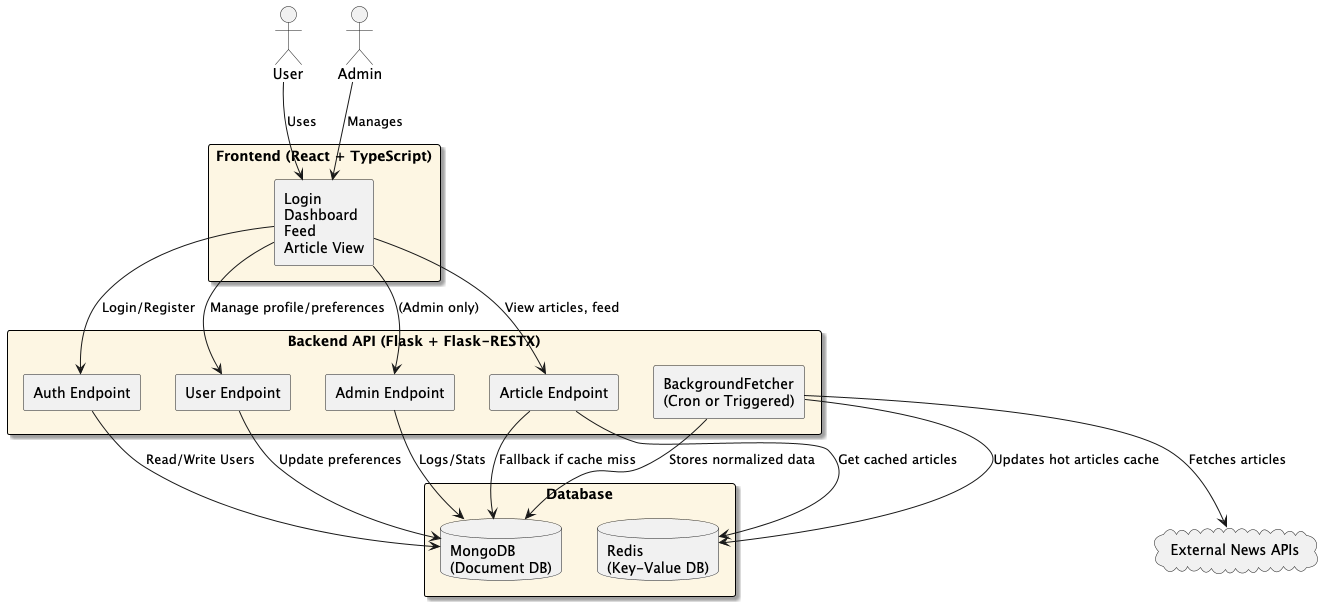
\includegraphics[width=1.1\textwidth]{chapters/chapter_03/system-architecture-smart-news-aggregator}
    \caption{System Architecture}
    \label{fig:system-architecture-diagram}
\end{figure}

\subsection{Client Layer (Frontend)}\label{subsec:client-layer-frontend}

At the forefront is the \textbf{Client Layer}, which consists of a web-based frontend developed using React and TypeScript.
This layer handles the user interface, manages routing, and communicates with the backend API through Axios.
JWT tokens are stored in the browser’s localStorage for session management.
Users interact with interfaces such as login, registration, the personalized news feed, article detail views, and, for administrators, a dedicated dashboard.

\subsection{Application Layer (Flask Backend)}\label{subsec:application-layer-flask-backend}

The \textbf{Application Layer} is built on Flask with Flask-RESTX to expose RESTful endpoints in a modular architecture.
This layer is responsible for authenticating users using asymmetric JWT (RS256), routing client requests to appropriate service handlers, and managing background tasks like scheduled fetching of articles.
It includes modules like auth\_endpoint, user\_endpoint, article\_endpoint, and admin\_endpoint, as well as libraries for handling authentication keys and logging system events into MongoDB\@.

\subsection{Data Layer}\label{subsec:data-layer}

The \textbf{Data Layer} integrates two complementary NoSQL technologies.
MongoDB, as a document-oriented database, is used to store structured collections such as users, articles, comments, preferences, and system logs.
It supports advanced aggregation pipelines and enables efficient historical analysis.
Redis, on the other hand, serves as a key-value store optimized for performance.
It caches the latest articles, manages trending topics, and supports rate limiting.
Redis ensures low-latency data access and reduces the load on MongoDB for repetitive queries.

\subsection{External APIs Layer}\label{subsec:external-apis-layer}

At the periphery, the \textbf{External APIs Layer} includes third-party news services like MediaStack, CurrentsAPI, NewsData, the New York Times API, and the Guardian API\@.
A background fetcher service, either scheduled or triggered, connects to these APIs, retrieves articles, normalizes the data, and saves the cleaned results into MongoDB\@.
This ensures that the content database is continuously updated with fresh news.

\vspace{2cm}

The data flow follows a secure and performance-driven path.
When a user logs in, they are authenticated via JWT, and the token is returned in the Authorization header.
The frontend then retrieves the latest articles by calling the /article/latest endpoint.
If the content is cached in Redis, it is served directly; otherwise, Flask queries MongoDB. Meanwhile, the background fetcher periodically updates the article repository.
Personalized recommendations are generated by combining user preferences with MongoDB aggregations and Redis-cached data.
Administrators can monitor platform activity and user engagement via metrics obtained through aggregation queries stored in MongoDB\@.

\section{UML Class Diagram}\label{sec:uml-class-diagram}

\begin{figure}[!h]
    \centering
    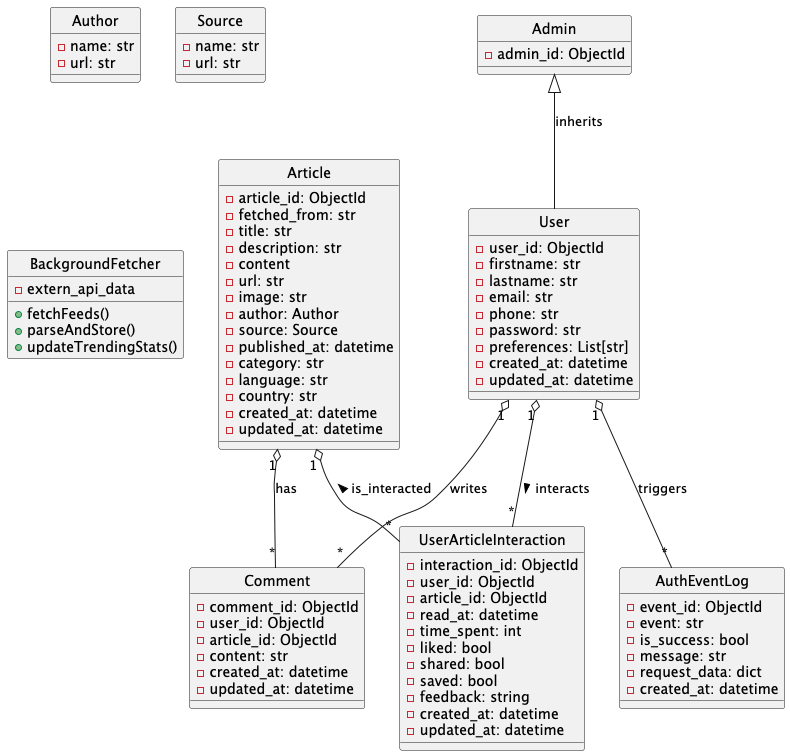
\includegraphics[width=1\textwidth]{chapters/chapter_03/uml-class-diagram}
    \caption{Use Case Diagram: Systen}
    \label{fig:uml-class-diagram}
\end{figure}




\section{UI Wireframes and Mockups}\label{sec:ui-wireframes-and-mockups}

\subsection{Authentication Screens}\label{subsec:authentication-screens}

For registered new user and login:

\begin{figure}[!h]
    \centering
    \begin{minipage}{0.48\linewidth}
        \centering
        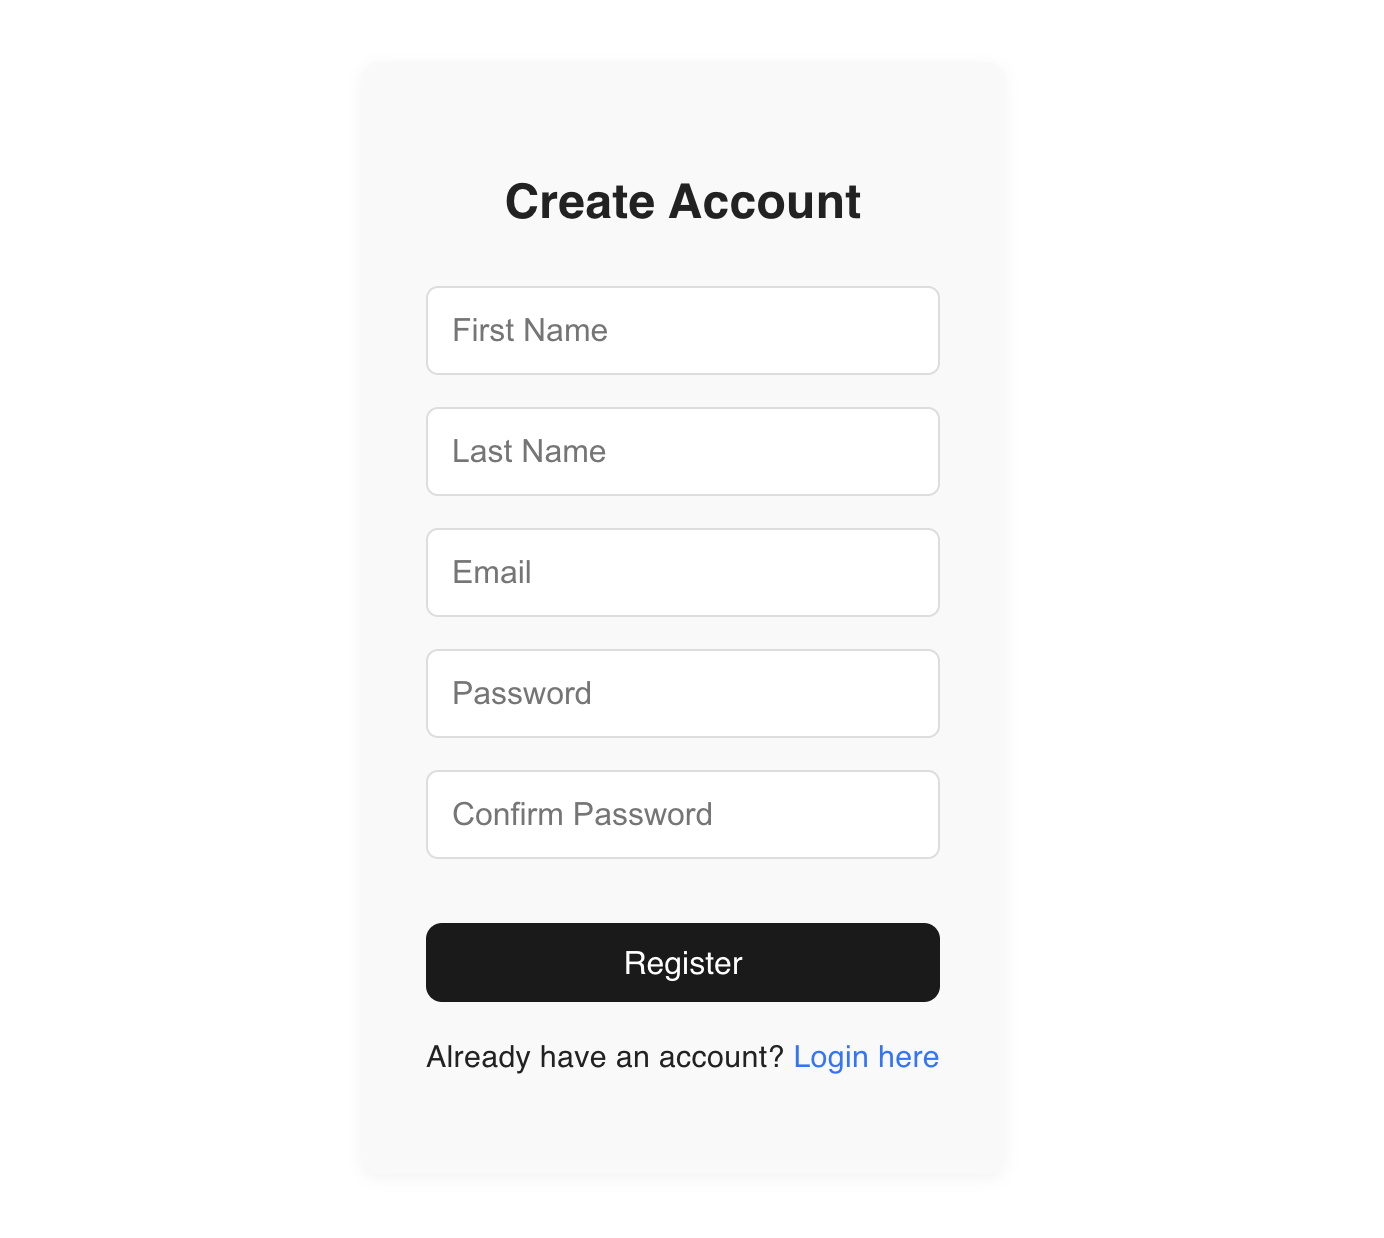
\includegraphics[width=1\textwidth]{chapters/chapter_03/page/auth/register-page}
        \caption{Authentication screens: registration page}
        \label{fig:registration-wireframes}
    \end{minipage}
    \hfil
    \begin{minipage}{0.48\linewidth}
        \centering
        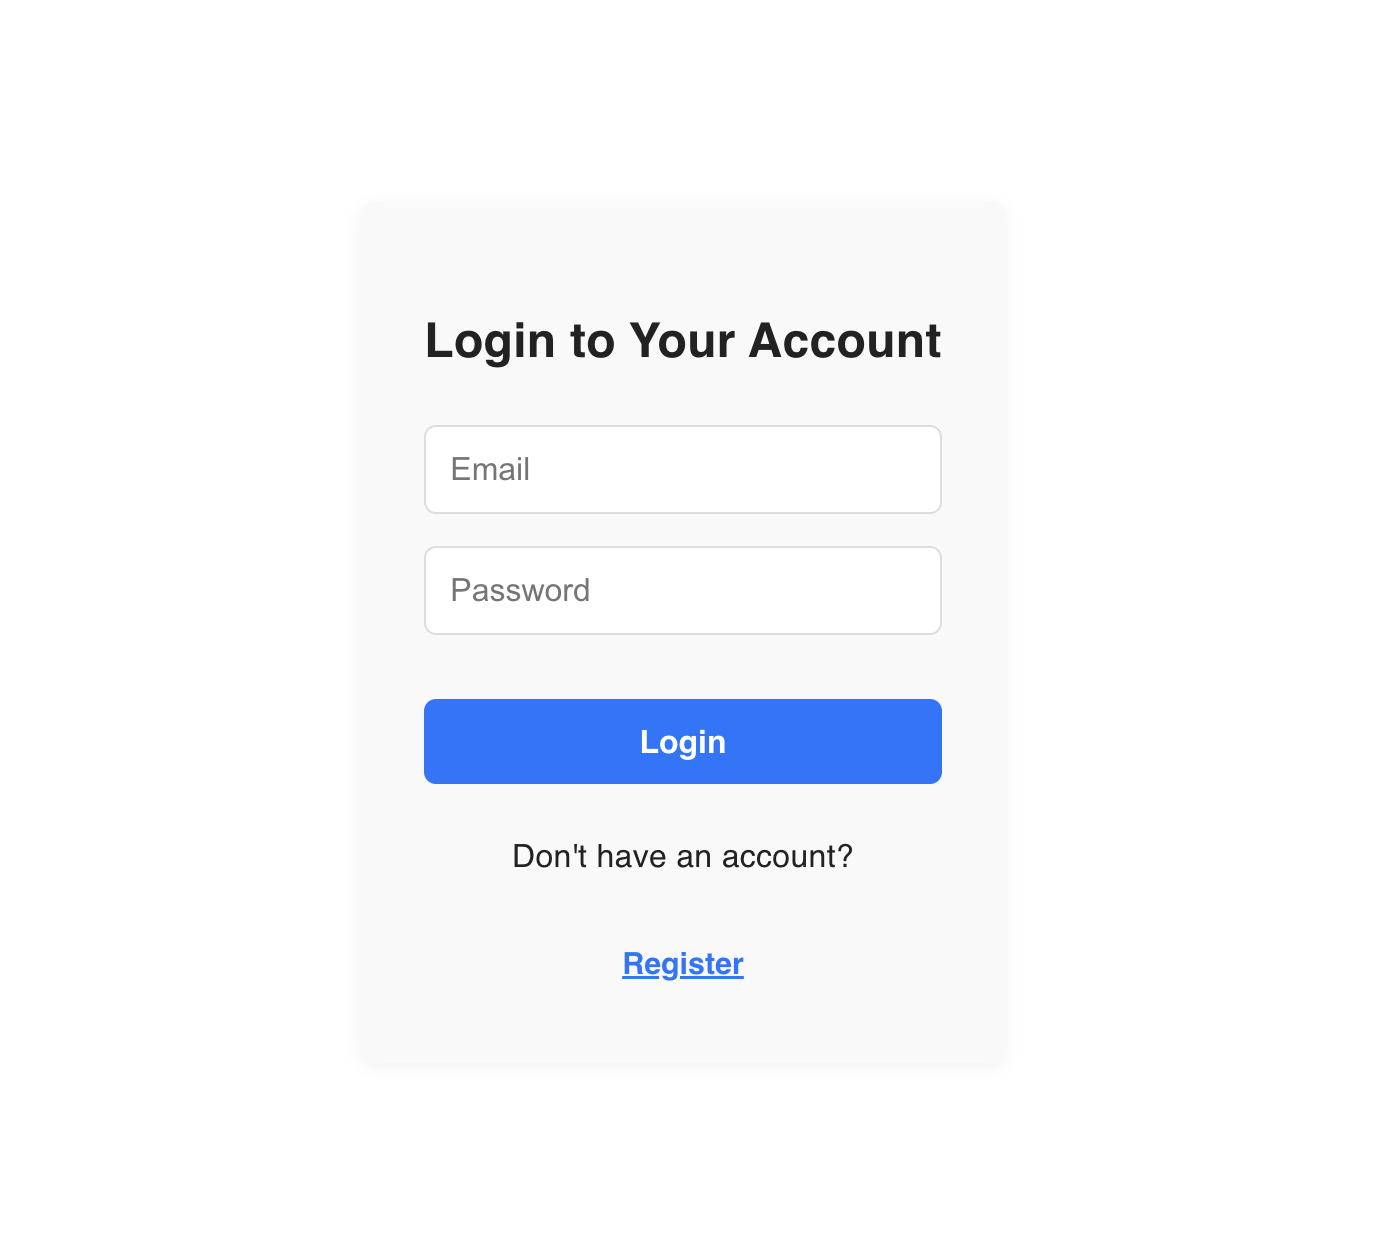
\includegraphics[width=1\textwidth]{chapters/chapter_03/page/auth/login-page}
        \caption{Authentication screens: login page}
        \label{fig:login-wireframes}
    \end{minipage}
\end{figure}


\subsection{User Screens}\label{subsec:user-screens}

For see user all user information.
It's not possible for user with role "user" to modify status and role.

\begin{figure}[!h]
    \centering
    \begin{minipage}{0.48\linewidth}
        \centering
        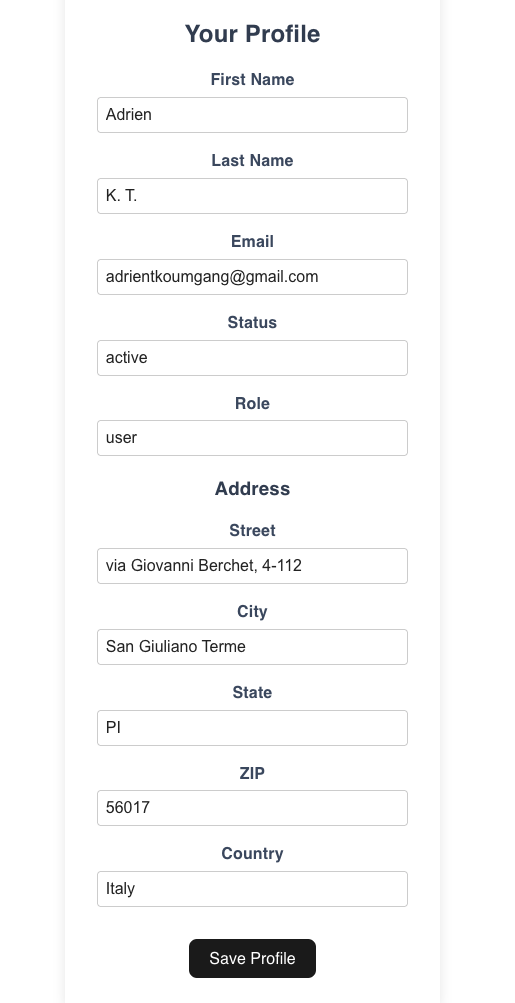
\includegraphics[width=0.8\textwidth]{chapters/chapter_03/page/user/profile-page}
        \caption{User screens: profile page}
        \label{fig:profile-wireframes}
    \end{minipage}
    \hfil
    \begin{minipage}{0.48\linewidth}
        \centering
        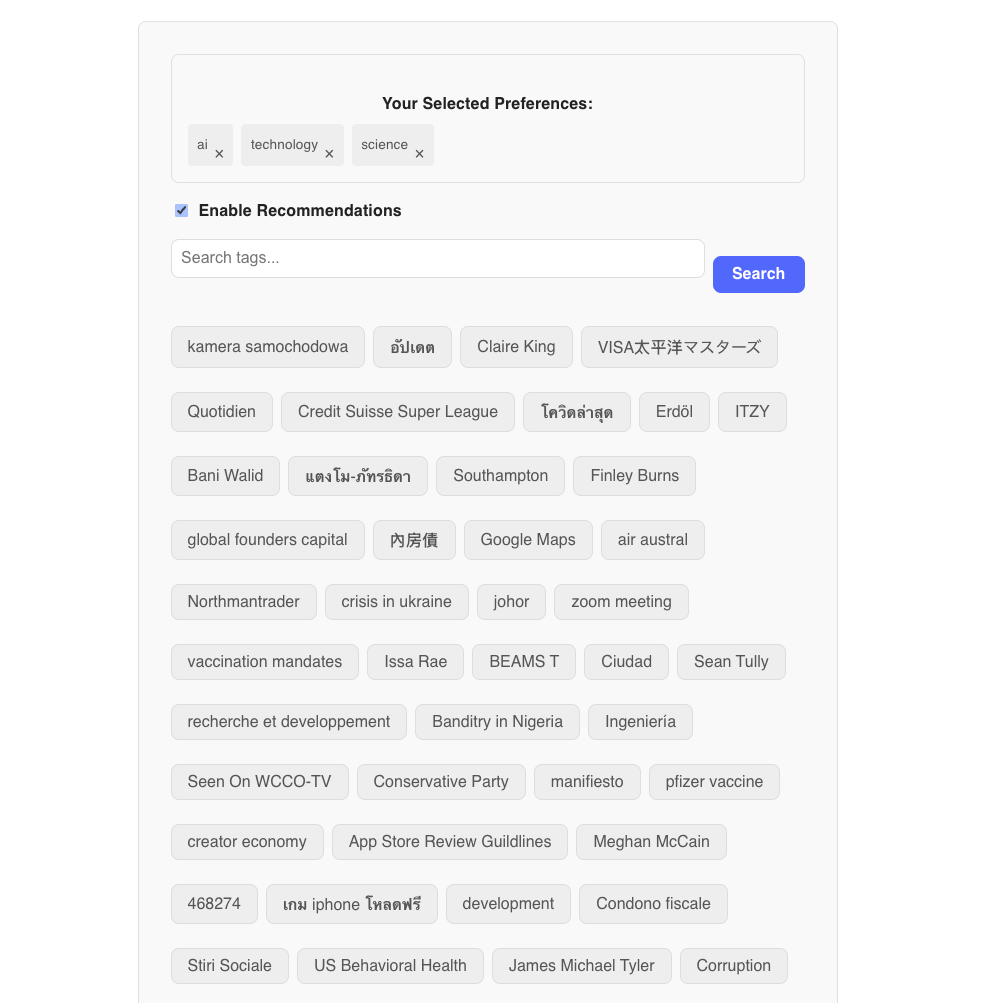
\includegraphics[width=1.2\textwidth]{chapters/chapter_03/page/user/settings-page}
        \caption{User screens: settings page}
        \label{fig:settings-wireframes}
    \end{minipage}
\end{figure}


\begin{figure}[!h]
    \centering
    \begin{minipage}{0.48\linewidth}
        \centering
        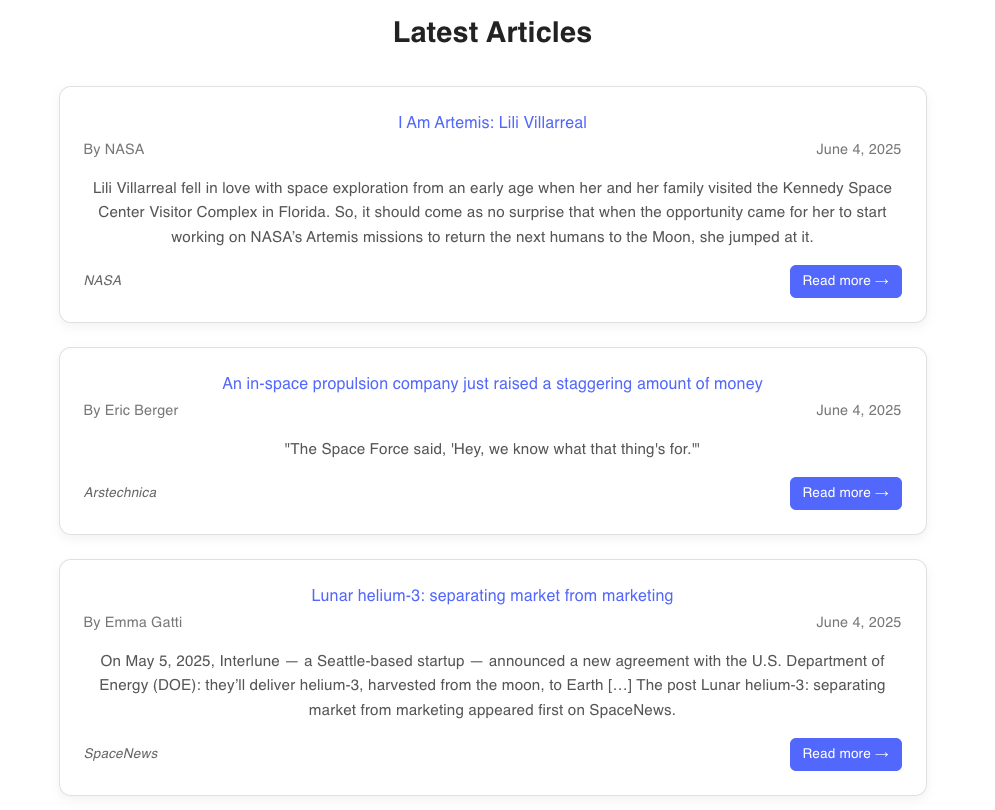
\includegraphics[width=1\textwidth]{chapters/chapter_03/page/user/latest-page}
        \caption{User screens: latest page}
        \label{fig:latest-wireframes}
    \end{minipage}
    \hfil
    \begin{minipage}{0.48\linewidth}
        \centering
        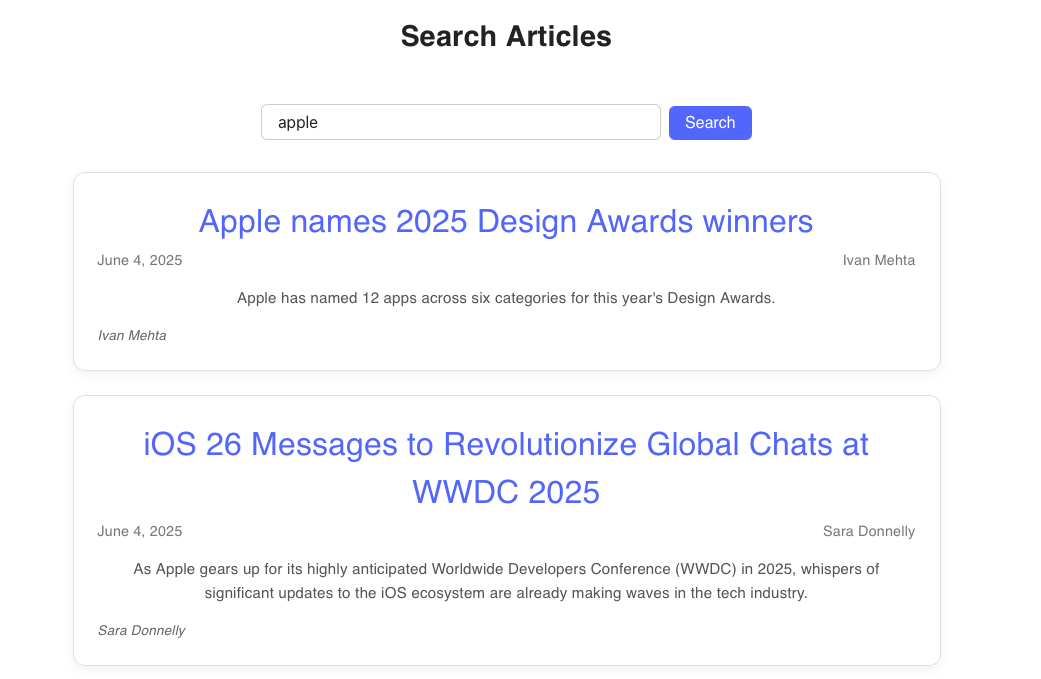
\includegraphics[width=1\textwidth]{chapters/chapter_03/page/user/search-page}
        \caption{User screens: Search page}
        \label{fig:search-wireframes}
    \end{minipage}
\end{figure}


\begin{figure}[!h]
    \centering
    \begin{minipage}{0.48\linewidth}
        \centering
        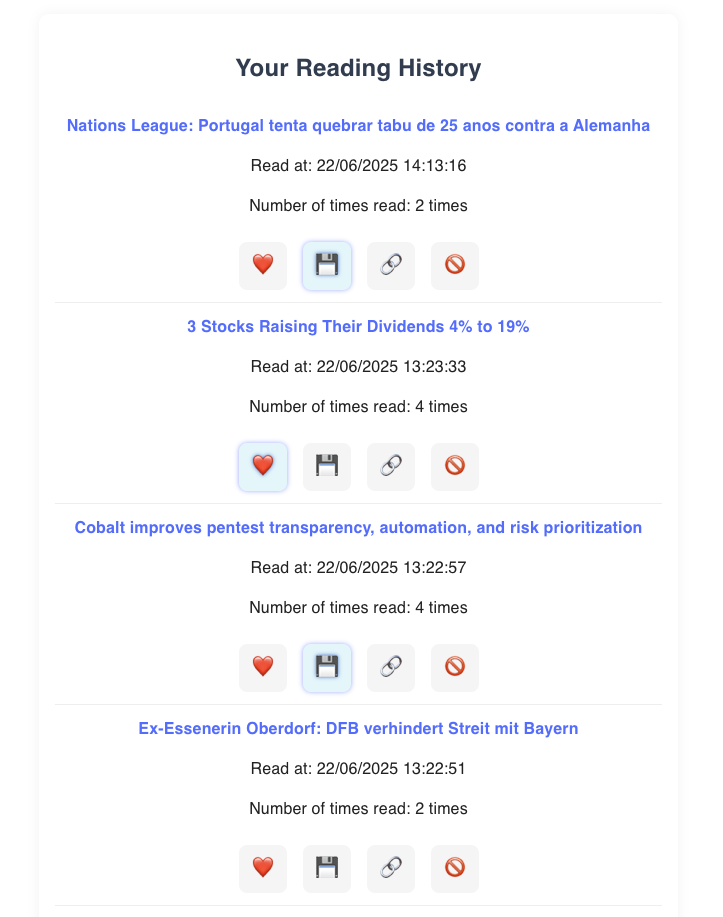
\includegraphics[width=1\textwidth]{chapters/chapter_03/page/user/history-page}
        \caption{User screens: History page}
        \label{fig:history-wireframes}
    \end{minipage}
    \hfil
    \begin{minipage}{0.48\linewidth}
        \centering
        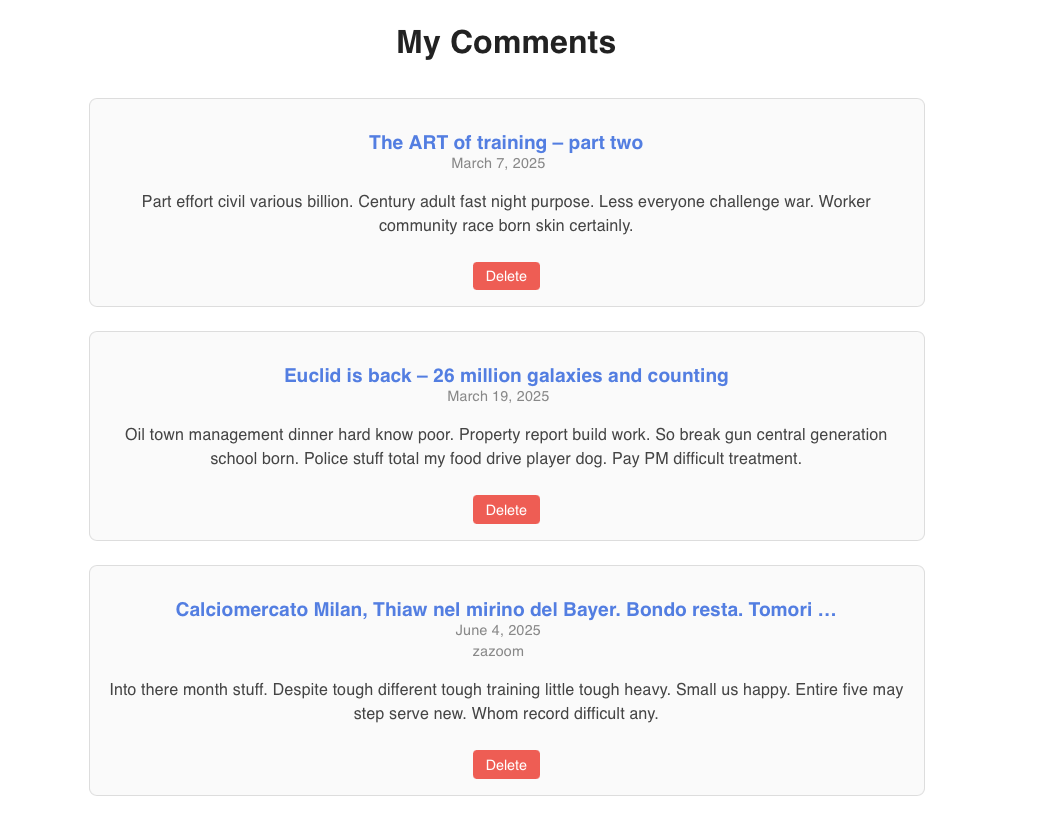
\includegraphics[width=1\textwidth]{chapters/chapter_03/page/user/comments-page}
        \caption{User screens: Comments page}
        \label{fig:comments-wireframes}
    \end{minipage}
\end{figure}



\begin{figure}[!h]
    \centering
    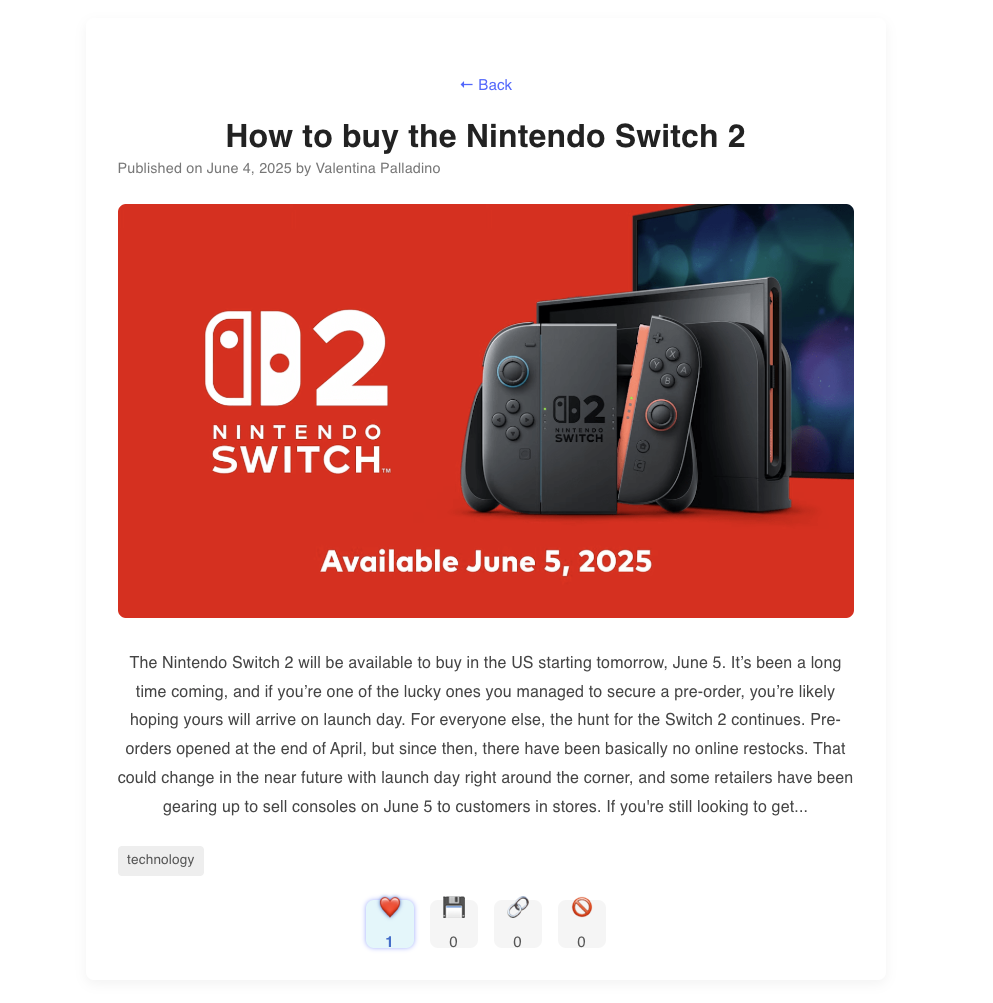
\includegraphics[width=0.7\textwidth]{chapters/chapter_03/page/user/article-details-page}
    \caption{User screens: articles details page}
    \label{fig:articles-details-wireframes}
\end{figure}


\subsection{Admin Screens}\label{subsec:admin-screens}

\begin{figure}[!h]
    \centering
    \begin{minipage}{0.48\linewidth}
        \centering
        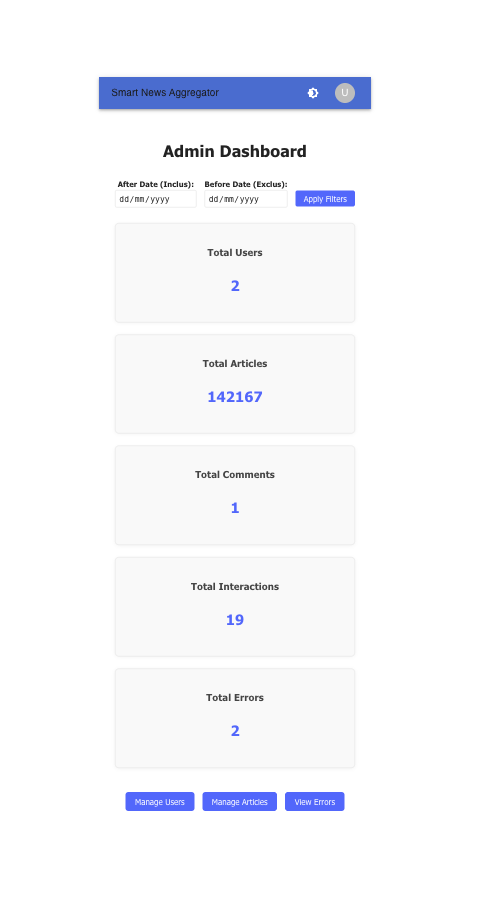
\includegraphics[width=1\textwidth]{chapters/chapter_03/page/admin/admin-dashboard-page}
        \caption{Admin screens: admin dashboard page}
        \label{fig:admin-dashboard-wireframes}
    \end{minipage}
    \hfil
    \begin{minipage}{0.48\linewidth}
        \centering
        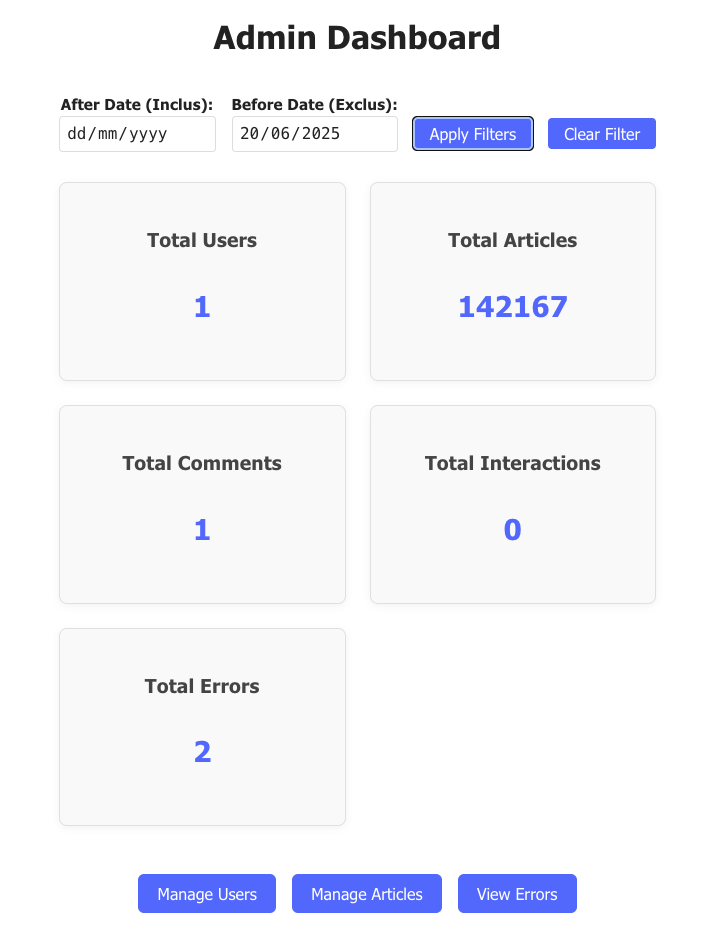
\includegraphics[width=1\textwidth]{chapters/chapter_03/page/admin/admin-dashboard-page-2}
        \caption{Admin screens: admin dashboard page}
        \label{fig:admin-dashboard-2-wireframes}
    \end{minipage}
\end{figure}


\begin{figure}[!h]
    \centering
    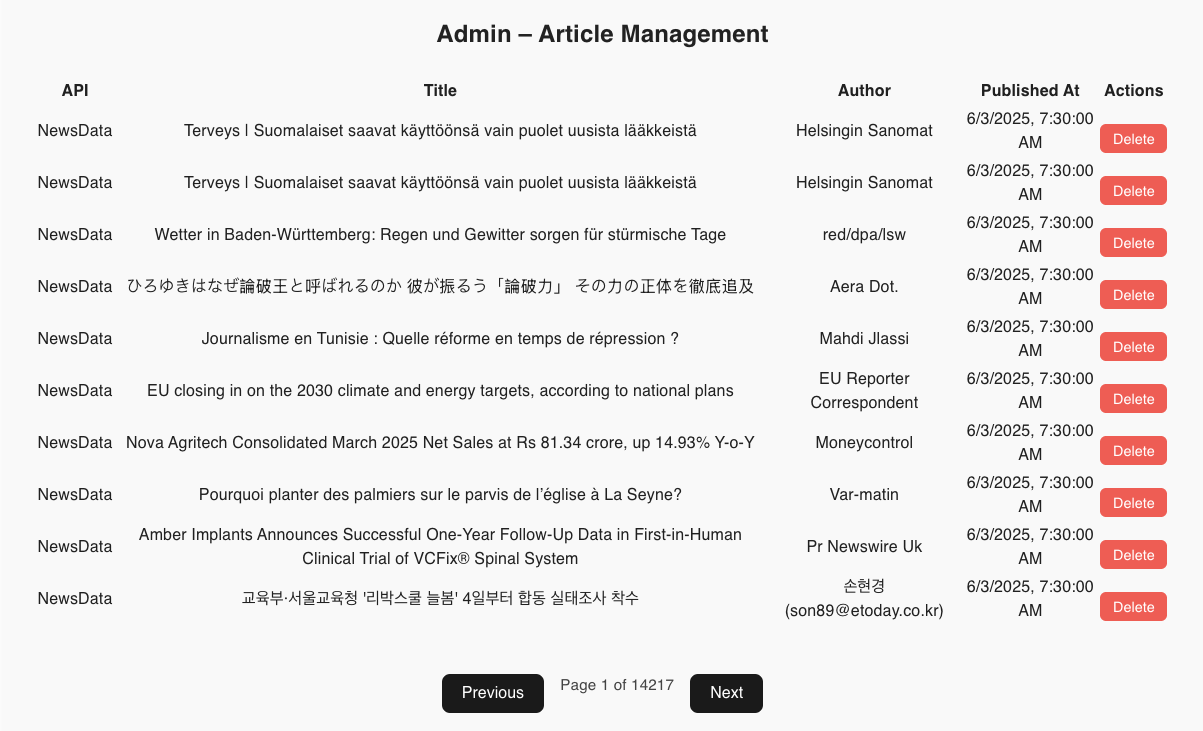
\includegraphics[width=0.7\textwidth]{chapters/chapter_03/page/admin/admin-articles-page}
    \caption{Admin screens: admin articles page}
    \label{fig:admin-articles-wireframes}
\end{figure}

\begin{figure}[!h]
    \centering
    \begin{minipage}{0.48\linewidth}
        \centering
        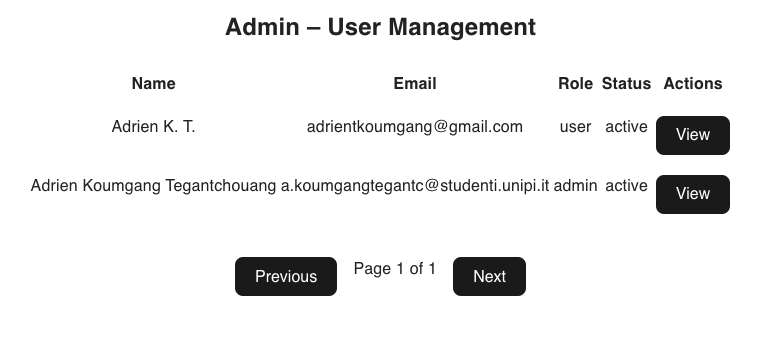
\includegraphics[width=1\textwidth]{chapters/chapter_03/page/admin/admin-users-page}
        \caption{Admin screens: admin users page}
        \label{fig:admin-users-wireframes}
    \end{minipage}
    \hfil
    \begin{minipage}{0.48\linewidth}
        \centering
        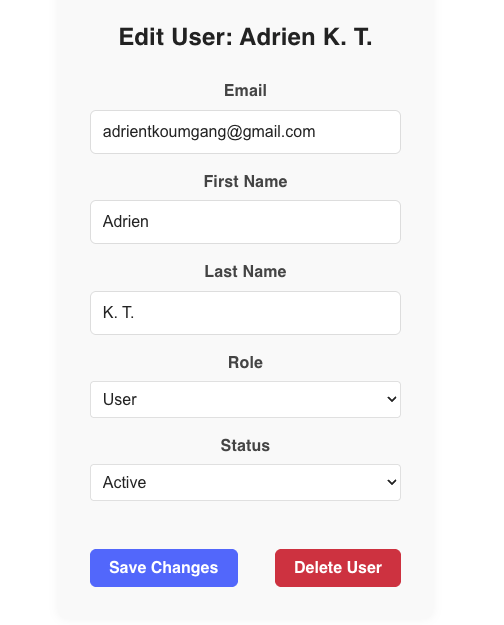
\includegraphics[width=1\textwidth]{chapters/chapter_03/page/admin/admin-user-details-page}
        \caption{Admin screens: admin user details page}
        \label{fig:admin-user-details-wireframes}
    \end{minipage}
\end{figure}


\begin{figure}[!h]
    \centering
    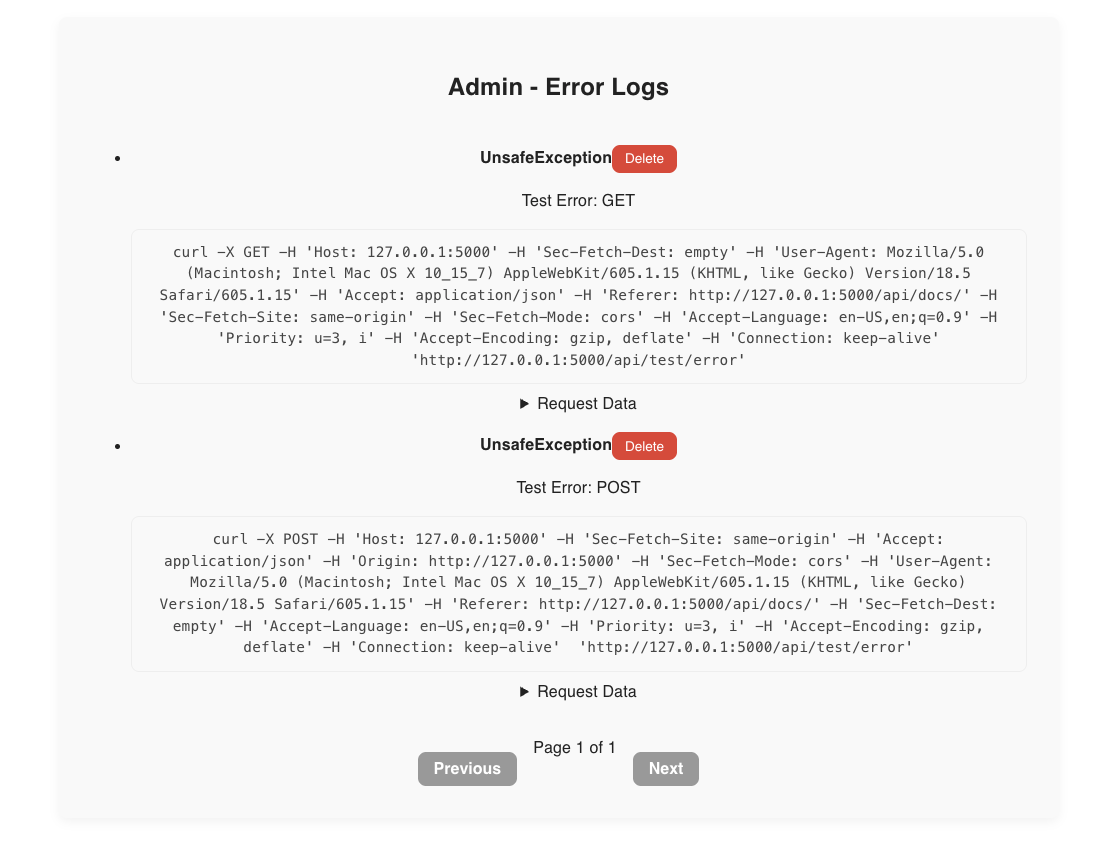
\includegraphics[width=0.7\textwidth]{chapters/chapter_03/page/admin/admin-error-logs-page}
    \caption{Admin screens: admin error logs page}
    \label{fig:admin-error-logs-wireframes}
\end{figure}





% Conclusion
    % \include{chapters/chapter_07}


    \bibliographystyle{splncs03}
    \bibliography{bibliography}
    % \printbibliography


% acknowledgement
    %! Author = adrienkoumgangtegantchouang
%! Date = 07/06/25


\chapter*{Acknowledgments}\label{ch:acknowledgments}


I thank God who gave me the strength to do this project.



    %! Author = adrienkoumgangtegantchouang
%! Date = 07/06/25



\end{document}
